\chapter{Étude préalable}
\fancyhead[L]{\leftmark}

%====================================================
%====================================================
\section{Introduction}

Ce chapitre présente l’étude préalable du projet \textit{SecureRAG Hub}. Il situe le projet dans son contexte, formule sa problématique, fixe ses objectifs, définit les concepts mobilisés, et analyse les solutions existantes pour justifier la solution proposée.

L’enrichissement bibliographique de cette étude s’appuie sur trois familles de références complémentaires. La première regroupe les travaux scientifiques relatifs aux modèles de langage, aux hallucinations et au RAG, notamment les contributions fondatrices sur les Transformers, les modèles de fondation et la génération augmentée par récupération \cite{vaswani_transformer_2017,bommasani_foundation_models_2021,lewis_rag_2020,gao_rag_survey_2024,ji_hallucination_survey_2023}. La deuxième famille réunit les référentiels de gouvernance, de sécurité et d’industrialisation, tels que le NIST AI RMF, le NIST SSDF, SLSA, OWASP LLM Top 10 et les recommandations Kubernetes/CIS \cite{nist_ai_rmf_2023,nist_ssdf_800_218,slsa_spec_v1,owasp_llm_top10_2025,cis_kubernetes_benchmark,k8s_pod_security_standards}. La troisième famille comprend les documentations officielles des solutions étudiées afin de comparer leur positionnement réel : ChatGPT Enterprise, Microsoft Copilot Studio, Amazon Q Business, Google Gemini Enterprise Agent Platform, IBM watsonx Assistant, Rasa, Botpress, LangChain et LangGraph \cite{openai_enterprise_admin_2026,microsoft_copilot_studio_2026,aws_q_business_2026,google_agent_platform_2026,ibm_watsonx_2026,rasa_docs_2026,botpress_docs_2026,langchain_retrieval_2026,langgraph_agentic_rag_2026}.


\textit{SecureRAG Hub} s’inscrit dans un contexte marqué par l’essor de l’intelligence artificielle générative, des assistants conversationnels métiers et des architectures cloud native. Les organisations cherchent aujourd’hui à exploiter des chatbots capables d’assister les utilisateurs, d’accéder à des connaissances internes et de simplifier certains processus. Cette tendance est documentée par les rapports récents sur l’adoption de l’IA, qui soulignent à la fois la diffusion rapide des usages génératifs et la difficulté de passer d’expérimentations isolées à des systèmes gouvernés et mesurables \cite{stanford_ai_index_2025,mckinsey_state_ai_2025}. Cependant, ces usages soulèvent des enjeux concrets de sécurité, de gouvernance, de traçabilité et de maîtrise du cycle de déploiement, en particulier face aux risques de prompt injection, de fuite d’information, de mauvaise gestion des permissions et de vulnérabilités de la chaîne logicielle \cite{owasp_llm_top10_2025,nist_ai_rmf_2023,slsa_spec_v1}.

Le projet ne se limite donc pas à la réalisation d’un chatbot. Il propose une plateforme sécurisée et industrialisée, combinant portail web, services applicatifs, architecture microservices, intelligence artificielle préparée, déploiement Kubernetes et chaîne DevSecOps. L’objectif est de construire une solution démontrable et traçable, capable d'évoluer, capable d’accueillir progressivement des capacités RAG et LLM plus avancées.

Le chapitre traite, dans cet ordre, le cadre général du projet, son contexte institutionnel, les concepts techniques clés, l’analyse de l’existant, la solution proposée ainsi que la méthodologie de conception retenue.
%====================================================
\section{Cadre général du projet}

\subsection{Cadre du projet}

\textit{SecureRAG Hub} est une plateforme production-like de chatbots métiers sécurisés, réalisée dans le cadre d’un Projet de Fin d’Études de niveau Master DSIR. Elle répond à une problématique actuelle : permettre à une organisation de déployer des assistants spécialisés par domaine métier, tout en maîtrisant les accès, la traçabilité, les artefacts logiciels et les conditions de déploiement.

La plateforme repose sur une architecture modulaire combinant un portail web Laravel Blade, des services applicatifs métiers, un socle Kubernetes local fondé sur \texttt{kind}, une registry cluster-reachable, une chaîne DevSecOps pilotée par Jenkins et des mécanismes de sécurisation de la supply chain logicielle. Cette structuration s’inscrit dans les recommandations relatives aux architectures microservices sécurisées, au développement logiciel sécurisé et à la provenance des artefacts \cite{nist_sp_800_204,nist_ssdf_800_218,slsa_spec_v1,sigstore_ccs_2022}.

Le scénario retenu est qualifié de \textit{production-like}. Il ne prétend pas remplacer une infrastructure cloud managée de production, mais il permet de démontrer localement les propriétés essentielles d’une plateforme moderne : déploiement par digest immuable, validation runtime des images exécutées, contrôles Kubernetes, génération de rapports de sécurité, preuves de supply chain et constitution d’un support pack final.

Dans cette version, les capacités IA/RAG sont traitées comme une extension architecturale préparée, mais non comme une dépendance obligatoire du scénario principal. Cette décision permet de stabiliser la démonstration et de concentrer l’évaluation sur la gouvernance, la sécurité, l’industrialisation et la preuve d’exécution.

\subsection{Motivations du projet}

Le choix de ce projet est motivé par la convergence de plusieurs tendances.

La première concerne l’adoption rapide de l’intelligence artificielle générative dans les organisations. Les utilisateurs attendent désormais des outils capables de répondre rapidement à des questions, d’assister les tâches métiers et de simplifier l’accès à l’information. Cette attente dépasse le cadre expérimental : elle s’inscrit dans une dynamique de transformation numérique où les assistants deviennent des interfaces naturelles d’accès aux connaissances internes.

La deuxième motivation est liée à la sécurité. Un chatbot d’entreprise peut manipuler des informations sensibles, telles que des données RH, des demandes internes, des incidents techniques, des documents confidentiels ou des traces d’audit. Il ne suffit donc pas de produire une réponse : il faut aussi contrôler les accès, journaliser les usages, isoler les domaines métiers et documenter les preuves techniques.

La troisième motivation relève de l’industrialisation. Une solution moderne ne doit pas uniquement fonctionner sur le poste du développeur. Elle doit pouvoir être testée, scannée, conteneurisée, signée, déployée et validée de manière reproductible. Cette exigence est d’autant plus importante dans un projet de fin d’études, où la crédibilité technique repose aussi sur la capacité à démontrer le fonctionnement réel des composants.

Enfin, ce projet permet de couvrir un périmètre technique cohérent avec un Master DSIR : développement web, architecture microservices, APIs REST, Docker, Kubernetes, Jenkins, sécurité applicative, sécurité cluster, supply chain logicielle et documentation de preuve.

\subsection{Problématique}

Les organisations souhaitent de plus en plus intégrer des assistants conversationnels dans leurs processus internes : ressources humaines, support informatique, assistance documentaire, conformité, audit ou support métier. Cependant, l’intégration directe de chatbots non gouvernés soulève plusieurs risques :

\begin{itemize}
    \item absence de contrôle précis sur les accès et les rôles ;
    \item manque de traçabilité des conversations ;
    \item difficulté à isoler les domaines métiers ;
    \item exposition potentielle de données sensibles ;
    \item absence de preuves sur les images réellement déployées ;
    \item difficulté à démontrer la fiabilité de la chaîne CI/CD ;
    \item dépendance excessive à des services externes ou à des modèles non maîtrisés.
\end{itemize}

La difficulté principale ne réside donc pas uniquement dans la génération de réponses par un modèle d’intelligence artificielle, mais dans la capacité à encadrer ces réponses, contrôler les accès, tracer les usages et déployer la plateforme de manière sécurisée et reproductible.

La problématique centrale du projet peut être formulée comme suit :

\begin{quote}
Comment concevoir une plateforme de chatbots métiers sécurisés, démontrable localement, gouvernée par rôles, industrialisée par une chaîne DevSecOps et prête à évoluer vers une intégration RAG complète ?
\end{quote}

\subsection{Objectifs du projet}
Afin d’ancrer la problématique dans une logique de recherche appliquée, trois questions directrices peuvent être retenues. Premièrement, comment organiser l’architecture applicative et le contrôle d’accès pour éviter qu’un chatbot métier ne devienne un point d’exposition des données sensibles ? Deuxièmement, quels contrôles DevSecOps permettent de relier le code source, l’image conteneurisée, le digest déployé et la preuve runtime ? Troisièmement, comment préparer une intégration RAG sans présenter comme opérationnel un moteur IA qui n’est pas encore validé dans le scénario officiel ? Ces questions relient la gouvernance RBAC \cite{sandhu_rbac_1996}, les stratégies de sécurité microservices \cite{nist_sp_800_204}, les recommandations de développement sécurisé \cite{nist_ssdf_800_218} et les travaux sur le RAG et les hallucinations \cite{lewis_rag_2020,gao_rag_survey_2024,ji_hallucination_survey_2023}.

\subsection{Hypothèses de travail}

L’étude préalable peut être structurée autour de trois hypothèses de travail :
\begin{itemize}
    \item \textbf{H1 — Gouvernance applicative.} Une plateforme de chatbots métiers devient plus défendable lorsqu’elle sépare explicitement les rôles, les permissions, les domaines métier et les traces d’audit, conformément aux principes du RBAC \cite{sandhu_rbac_1996}.
    \item \textbf{H2 — Industrialisation vérifiable.} Une chaîne DevSecOps intégrant tests, SAST, détection de secrets, scan de vulnérabilités, SBOM, signature et promotion par digest améliore la reproductibilité et la confiance dans les artefacts déployés \cite{nist_ssdf_800_218,slsa_spec_v1,cyclonedx_spec,sigstore_ccs_2022}.
    \item \textbf{H3 — IA préparée mais maîtrisée.} Le fait de préparer l’intégration RAG sans rendre le scénario officiel dépendant d’un LLM réel limite les risques de démonstration et renforce la distinction entre résultats validés et perspectives de recherche \cite{lewis_rag_2020,gao_rag_survey_2024}.
\end{itemize}



Les objectifs du projet sont à la fois applicatifs, architecturaux, sécuritaires et DevSecOps.

Sur le plan applicatif, le projet vise à :

\begin{itemize}
    \item proposer un portail web \textit{user/admin} basé sur Laravel Blade ;
    \item gérer les utilisateurs, les rôles et les permissions ;
    \item gérer un catalogue de chatbots métiers ;
    \item préparer les conversations et l’historique ;
    \item superviser les incidents et les traces de sécurité ;
    \item exposer des APIs REST versionnées pour les services applicatifs ;
    \item structurer une base évolutive capable d’accueillir ultérieurement une orchestration conversationnelle plus avancée.
\end{itemize}

Sur le plan DevSecOps, le projet vise à :

\begin{itemize}
    \item automatiser les tests et les contrôles de sécurité ;
    \item utiliser Jenkins comme chaîne officielle de CI/CD ;
    \item construire et publier des images conteneurisées ;
    \item générer des SBOM ;
    \item signer et vérifier les images ;
    \item promouvoir les images par digest ;
    \item déployer la plateforme sur un cluster Kubernetes local ;
    \item appliquer des contrôles de sécurité Kubernetes ;
    \item générer des preuves techniques exploitables en soutenance.
\end{itemize}

\subsection{Périmètre du projet}

Le périmètre principal du projet couvre la conception et la réalisation d’une plateforme de chatbots métiers sécurisés. Il inclut le portail web, la gestion des utilisateurs et des rôles, le catalogue de chatbots, les services applicatifs, le déploiement Kubernetes local et la chaîne DevSecOps.

Le projet couvre également la production de preuves techniques : rapports de tests, résultats de scans, manifests Kubernetes, support pack, runbooks et documentation mémoire. Cette dimension est essentielle, car elle permet de démontrer le fonctionnement du système et sa qualité d'industrialisation.

En revanche, certains éléments ne font pas partie du périmètre principal de cette version. Le projet ne vise ni à entraîner un modèle d’intelligence artificielle, ni à développer un moteur RAG complet, ni à exploiter un LLM réel en production. Ces éléments sont considérés comme des perspectives d’évolution. La version actuelle privilégie une architecture prête à les accueillir, avec un scénario stable, maîtrisé et démontrable.

\subsection{Clarification du périmètre IA/RAG}

Dans ce projet, l’intelligence artificielle est principalement traitée comme une capacité d’intégration architecturale. Le système est conçu pour accueillir des composants IA, mais le développement d’un modèle LLM réel ou d’un moteur RAG complet ne constitue pas l’objectif principal de cette version.

Cette distinction est essentielle pour éviter toute ambiguïté. Le projet démontre la gouvernance, la sécurité, l’architecture microservices, le portail, les APIs et la chaîne DevSecOps. L’intégration d’un moteur IA réel reste néanmoins possible grâce aux contrats, aux adaptateurs et aux composants prévus dans l’architecture.

Ainsi, la valeur actuelle de \textit{SecureRAG Hub} réside moins dans la performance conversationnelle brute que dans la capacité de la plateforme à encadrer, sécuriser, tracer et industrialiser les usages futurs de l’IA générative.

\subsection{Contraintes du projet}

Le projet doit respecter plusieurs contraintes :

\begin{itemize}
    \item rester démontrable dans un environnement local ou cloud léger ;
    \item ne pas exposer de secrets réels dans le dépôt ;
    \item distinguer clairement ce qui est réellement exécuté de ce qui est prêt à être exécuté ;
    \item ne pas dépendre d’un LLM réel pour le scénario officiel ;
    \item garantir la stabilité du mode production-like ;
    \item conserver une architecture lisible et défendable dans un mémoire de Master ;
    \item maintenir une cohérence entre les choix d’architecture, le périmètre réel du projet et les preuves disponibles.
\end{itemize}

\subsection{Limites identifiées}

Certaines limites sont assumées dans cette version. Le scénario officiel ne dépend pas d’un moteur LLM réel complet. Ce choix permet de sécuriser la démonstration et d’éviter qu’un problème de téléchargement de modèle, de ressources matérielles ou de disponibilité externe ne compromette la présentation.

Par ailleurs, certaines extensions avancées, comme GitOps complet, observabilité SRE enrichie, SOPS/age réellement opéré ou détection runtime de type Falco/Tetragon, sont préparées ou documentées, mais peuvent rester dépendantes de l’environnement. Ces limites ne sont pas masquées. Elles sont documentées afin de distinguer clairement l’état validé du projet, les éléments prêts à être rejoués et les composants dépendants de l’environnement.

%====================================================
\section{Cadre institutionnel du projet}

\subsection{Présentation générale}

Le projet \textit{SecureRAG Hub} est réalisé dans un cadre académique de Projet de Fin d’Études. Il s’inscrit dans une démarche d’ingénierie logicielle appliquée, avec un accent particulier sur la sécurité, l’industrialisation, la conteneurisation et la démonstration technique.

Dans cette perspective, le présent chapitre privilégie la présentation du contexte académique, du cadre de réalisation et des services fonctionnels visés, sans introduire d’informations organisationnelles non vérifiées. Si le mémoire final doit être rattaché à un organisme d’accueil précis, cette partie pourra être complétée à partir d’informations officiellement validées.

\subsection{Services concernés}

Les services fonctionnels simulés ou ciblés par la plateforme sont :

\begin{itemize}
    \item un service Ressources Humaines, représenté par un chatbot RH ;
    \item un service Support Informatique, représenté par un chatbot IT ;
    \item une équipe d’administration de plateforme ;
    \item une équipe sécurité chargée de l’audit, des incidents et des contrôles ;
    \item une chaîne DevSecOps responsable de la validation, du déploiement et des preuves techniques.
\end{itemize}

\subsection{Organisation fonctionnelle simplifiée}

L'organisation fonctionnelle de 	extit{SecureRAG Hub} peut être représentée de manière simplifiée comme suit :

\begin{figure}[htbp]
    \centering
    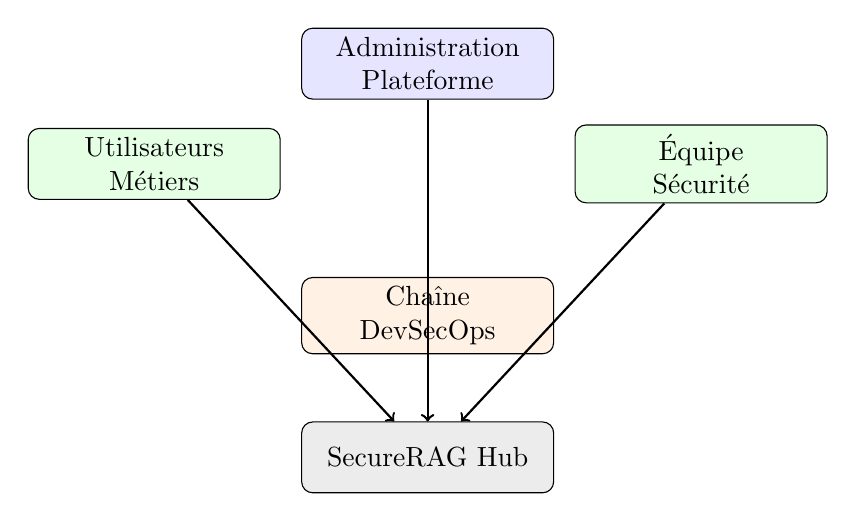
\begin{tikzpicture}[
        node distance=1.8cm,
        every node/.style={draw, rounded corners, align=center, minimum width=3.2cm, minimum height=0.9cm}
    ]
        \node[fill=blue!10] (admin) {Administration\\Plateforme};
        \node[fill=green!10, below left of=admin, xshift=-2.2cm] (users) {Utilisateurs\\Métiers};
        \node[fill=green!10, below right of=admin, xshift=2.2cm] (security) {Équipe\\Sécurité};
        \node[fill=orange!10, below of=admin, yshift=-1.4cm] (devsecops) {Chaîne\\DevSecOps};
        \node[fill=gray!15, below of=devsecops] (platform) {SecureRAG Hub};

        \draw[->, thick] (admin) -- (platform);
        \draw[->, thick] (users) -- (platform);
        \draw[->, thick] (security) -- (platform);
        \draw[->, thick] (devsecops) -- (platform);
    \end{tikzpicture}
    \caption{Organisation fonctionnelle simplifiée autour de SecureRAG Hub}
    \label{fig:organigramme_fonctionnel_securerag}
\end{figure}

%====================================================
\section{Contexte scientifique et technologique}

\subsection{Évolution récente des assistants conversationnels}

Les assistants conversationnels ont connu une évolution rapide, passant de systèmes à règles relativement rigides à des modèles capables de produire des réponses contextualisées, plus riches et plus naturelles. Cette évolution a été rendue possible par les progrès en traitement automatique du langage, en apprentissage profond et en puissance de calcul, en particulier depuis l’introduction de l’architecture Transformer et la généralisation des modèles de fondation \cite{vaswani_transformer_2017,bommasani_foundation_models_2021,stanford_ai_index_2025}.

Dans les organisations, cette transformation a modifié la manière de concevoir l’assistance numérique. Alors que les premiers chatbots étaient souvent limités à des FAQ ou à des scénarios fermés, les systèmes actuels ambitionnent de traiter des demandes variées, d’accéder à des bases documentaires internes et d’accompagner les utilisateurs dans des tâches professionnelles.

Cependant, plus les systèmes deviennent puissants et souples, plus les enjeux de fiabilité, de sécurité et de gouvernance deviennent importants. Une réponse linguistiquement convaincante ne garantit pas qu’elle soit correcte, autorisée ou conforme à un contexte métier donné. Les travaux sur les hallucinations montrent que les modèles génératifs peuvent produire des réponses fluides mais non fidèles aux sources ou au contexte fourni \cite{ji_hallucination_survey_2023}. Ce constat justifie l’émergence de plateformes structurées autour de principes de sécurité, de traçabilité et d’industrialisation \cite{nist_ai_rmf_2023,owasp_llm_top10_2025}.

\subsection{Enjeux de gouvernance et de sécurité}

L’intégration d’assistants conversationnels dans les environnements professionnels soulève des enjeux particuliers. Un chatbot connecté à des ressources internes peut devenir un point d’accès vers des données sensibles ou des processus critiques. Il ne suffit donc pas d’évaluer la qualité de ses réponses ; il faut aussi considérer qui l’utilise, dans quelles conditions, avec quelles permissions et selon quelles règles de journalisation.

La gouvernance des accès constitue ainsi un enjeu central. Dans un environnement multi-profils, tous les utilisateurs ne doivent pas disposer des mêmes droits ni du même niveau de visibilité sur les connaissances mobilisées. Les modèles RBAC restent adaptés à ce type de séparation, car ils associent les permissions à des rôles plutôt qu’à des utilisateurs isolés \cite{sandhu_rbac_1996}. À cela s’ajoutent les exigences d’auditabilité, de conformité et de traçabilité.

La sécurité doit également être pensée à plusieurs niveaux : sécurité applicative, sécurité des échanges, sécurité des images, sécurité des déploiements, sécurité des secrets et sécurité de la chaîne CI/CD. Ce constat renforce la pertinence d’une démarche DevSecOps intégrée au projet dès les premières phases de conception, conformément au NIST SSDF et aux pratiques de sécurisation de la chaîne d’approvisionnement logicielle \cite{nist_ssdf_800_218,slsa_spec_v1,ohm_supply_chain_attacks_2020}.

\subsection{Positionnement des plateformes RAG en entreprise}

Les approches de type RAG occupent aujourd’hui une place importante dans les usages professionnels des LLM. Elles répondent à une limite bien connue des modèles génératifs : leur tendance à produire des réponses plausibles mais non nécessairement ancrées dans les connaissances internes de l’organisation.

En réintroduisant une phase de recherche documentaire avant la génération, le paradigme RAG vise à améliorer la pertinence, la contextualisation et la vérifiabilité des réponses. Les travaux fondateurs de Lewis \textit{et al.} montrent l’intérêt d’associer mémoire paramétrique et mémoire non paramétrique, tandis que les études récentes distinguent des formes naïves, avancées et modulaires du RAG \cite{lewis_rag_2020,karpukhin_dpr_2020,gao_rag_survey_2024}. Toutefois, son intégration dans un cadre professionnel exige plus qu’une simple combinaison de recherche vectorielle et de génération de texte. Elle suppose une gestion rigoureuse des sources, des permissions, des traces, des politiques de sécurité et des mécanismes de déploiement.

Dans ce contexte, \textit{SecureRAG Hub} ne se positionne pas comme un moteur RAG finalisé, mais comme une plateforme prête à accueillir ce type de logique dans un cadre gouverné, sécurisé et industrialisé.

%====================================================
\section{Acteurs et scénarios d’usage}

\subsection{Acteurs du système}

Les principaux acteurs identifiés sont :

\begin{itemize}
    \item l’utilisateur RH ;
    \item l’utilisateur IT ;
    \item l’administrateur de plateforme ;
    \item l’administrateur sécurité ;
    \item la chaîne DevSecOps.
\end{itemize}

\subsection{Cas d’utilisation principaux}

Les cas d’utilisation majeurs du système peuvent être résumés comme suit :

\begin{itemize}
    \item se connecter au portail ;
    \item consulter les chatbots disponibles selon son rôle ;
    \item envoyer une requête à un chatbot métier ;
    \item consulter l’historique des conversations ;
    \item administrer les utilisateurs et les rôles ;
    \item superviser les événements de sécurité ;
    \item lancer, valider et documenter une chaîne de contrôle DevSecOps.
\end{itemize}

\subsection{Scénario métier 1 : consultation d’un chatbot RH}

Dans un premier scénario, un utilisateur appartenant au domaine RH accède au portail, s’authentifie, puis consulte le catalogue de chatbots autorisés. Il sélectionne le chatbot RH et soumet une question relative à une procédure interne. La plateforme transmet la demande au service concerné, applique les règles de sécurité prévues, puis retourne une réponse contrôlée. L’échange est ensuite journalisé afin de garantir la traçabilité du scénario.

\subsection{Scénario métier 2 : assistance support IT}

Dans un second scénario, un utilisateur du domaine IT se connecte au portail afin d’obtenir une assistance sur un incident courant. Il sélectionne le chatbot support IT, saisit sa requête et reçoit une réponse préparée selon les règles du système. Ce scénario permet de démontrer la spécialisation métier, l’isolation logique des usages et la capacité de la plateforme à supporter plusieurs assistants dans un même cadre gouverné.

\subsection{Scénario d’administration}

Dans un troisième scénario, un administrateur de plateforme accède aux fonctions de gestion. Il consulte la liste des utilisateurs, gère les rôles et supervise le catalogue de chatbots. Ce scénario met en évidence la séparation entre usage métier et administration, ainsi que la nécessité d’un contrôle d’accès fondé sur les rôles.

\subsection{Scénario de supervision sécurité}

Un administrateur sécurité consulte les événements de sécurité, les incidents et les traces disponibles. Ce scénario illustre l’importance de l’audit, de la journalisation et de la gouvernance dans une plateforme traitant des échanges sensibles.

%====================================================
%====================================================
\section{Concepts clés du projet}
\label{sec:concepts-cles}

SecureRAG~Hub n'est pas un seul outil ni une seule technologie. La plateforme
assemble plusieurs familles de concepts autour d'une exigence unique~: livrer
une chaîne production-like dont chaque étape peut être prouvée. On y trouve du
développement logiciel Laravel, une architecture en microservices, une
préparation IA et RAG, une chaîne DevSecOps pilotée par Jenkins, une
\emph{supply chain} logicielle signée, un cluster Kubernetes \emph{kind}
déployé sur VPS, des contrôles d'admission Kyverno, une détection runtime
Falco, des mécanismes de gestion des secrets, une couche de données
PostgreSQL avec sauvegarde, un dispositif d'observabilité
Prometheus--Loki--Grafana, et un \emph{support pack} final qui matérialise
les preuves.

Cette section définit chaque concept, précise son rôle exact dans
SecureRAG~Hub et donne un exemple d'utilisation, sans entrer dans une
classification de maturité (cette dimension est traitée ailleurs dans le
mémoire). L'objectif est de fournir au lecteur un vocabulaire commun pour
suivre les chapitres suivants.

% -------------------------------------------------------------
\subsection{Familles de concepts mobilisées}
\label{subsec:familles-concepts}

Le projet mobilise douze familles. Le \textbf{développement logiciel}
fournit le code applicatif Laravel, ses tests et sa documentation.
L'\textbf{architecture applicative} découpe le système en services REST
contractualisés. La famille \textbf{IA, LLM et RAG} pose les briques d'une
couche générative ancrée dans les documents internes. Le \textbf{DevOps} et
le \textbf{DevSecOps} industrialisent le cycle code--scan--build--release
sous l'autorité de Jenkins. La \textbf{supply chain} logicielle relie
chaque image OCI à un \emph{digest} immuable signé. \textbf{Kubernetes}
fournit la plateforme d'exécution, et la \textbf{sécurité Kubernetes}
durcit les pods à la conception. L'\textbf{admission control} valide
chaque manifest à son arrivée dans le cluster, tandis que la
\textbf{sécurité runtime} observe le comportement réel des charges de
travail. Les familles \textbf{secrets, données et résilience} d'une part,
et \textbf{observabilité et SRE} d'autre part, prennent en charge la
confidentialité, la continuité et la visibilité opérationnelle. La
dernière famille, \textbf{preuves et \emph{readiness}}, consolide les
artefacts produits par la chaîne en un livrable défendable.

% -------------------------------------------------------------
\subsection{Développement et architecture logicielle}
\label{subsec:concepts-developpement}

Le cœur applicatif repose sur Laravel et un découpage en cinq services
indépendants. Le portail web est une application MVC classique, dont les
vues sont rendues par le moteur de \emph{templating} Blade. Chaque service
expose une API REST documentée par un contrat et, pour les routes
publiques, par une description OpenAPI rangée dans
\texttt{docs/openapi/}. L'\emph{API Gateway} centralise l'entrée
utilisateur et le routage entre services. Les contrôleurs HTTP délèguent
aux \emph{models} Eloquent l'accès aux données, et le schéma relationnel
évolue par \emph{migrations} versionnées et \emph{seeders}, ce qui rend
l'état de la base reproductible.

L'authentification et l'autorisation sont gérées au niveau applicatif
par le service \texttt{auth-users-service}, qui implémente un RBAC orienté
métier. La base de données cible est PostgreSQL en mode production-like~;
SQLite reste utilisé en développement pour accélérer les itérations. Les
tests unitaires et fonctionnels sont exécutés par
\texttt{scripts/ci/run-tests.sh}, et un scénario de bout-en-bout est
fourni par \texttt{scripts/validate/e2e-functional-flow.sh}.

Le code est versionné dans Git, hébergé sur GitHub, et fusionné via des
\emph{Pull Requests} contrôlées par les vérifications CI. Les opérations
récurrentes (déploiement, rotation de secrets, restauration de
sauvegarde) sont décrites dans des \emph{runbooks} regroupés sous
\texttt{docs/runbooks/}, et l'architecture de la plateforme est tracée
dans \texttt{docs/architecture/} et \texttt{docs/devsecops/}.

% -------------------------------------------------------------
\subsection{Intelligence artificielle, LLM et RAG}
\label{subsec:concepts-ia}

L'intelligence artificielle générative est traitée comme une architecture
d'évolution. Un \emph{Large Language Model} (LLM) produit du texte à
partir d'un \emph{prompt}, lui-même précédé d'un \emph{prompt système} qui
fixe le rôle du chatbot et ses garde-fous. Deux risques propres à cette
classe de modèles sont identifiés et anticipés~: la \emph{prompt
injection}, dans laquelle une entrée utilisateur tente de modifier
l'instruction système, et l'\emph{hallucination}, qui désigne une réponse
plausible mais fausse. Le NLP intervient en amont du LLM pour normaliser
les entrées, détecter la langue et préparer la tokenisation.

Le \emph{Retrieval Augmented Generation} (RAG) ancre les réponses dans
une base documentaire propre à l'organisation. Cette base est
préalablement transformée en \emph{embeddings} (vecteurs denses) puis
indexée dans une base vectorielle telle que Qdrant, dont le manifeste est
posé dans \texttt{infra/k8s/base/qdrant/}. Un orchestrateur LLM compose
le \emph{prompt} final à partir des passages retrouvés et appelle le
modèle. Un \emph{security-auditor} IA vérifie les sorties avant retour à
l'utilisateur~; ce service peut s'appuyer sur un mécanisme de
\emph{LLM-as-judge}, où un second appel évalue la conformité de la
première réponse. Le pipeline RAG complet n'est pas exécuté dans le
scénario officiel actuel, mais ses services sont posés dans
\texttt{services/} avec leurs \texttt{Dockerfile}, leur namespace et
leur place dans la chaîne DevSecOps.

% -------------------------------------------------------------
\subsection{DevOps et DevSecOps}
\label{subsec:concepts-devsecops}

Le DevOps unifie développement et exploitation autour de la livraison
continue. Le DevSecOps y ajoute des contrôles de sécurité à chaque étape,
de sorte qu'aucune image ne soit livrée sans avoir traversé une série de
\emph{gates}. Dans SecureRAG~Hub, l'autorité CI/CD officielle est
Jenkins~: le \texttt{Jenkinsfile} de 218 lignes décrit le pipeline CI
(lint, tests, scans), et le \texttt{Jenkinsfile.cd} décrit la chaîne de
\emph{release} (scan, signature, promotion, attestation). Le contrôleur
Jenkins est lui-même protégé par un RBAC qui distingue lecteur,
contributeur et opérateur, et son intégration au dépôt SCM avec
\emph{webhook} fournit la preuve d'exécution réelle.

Trois \emph{gates} de sécurité statiques sont systématiques en CI~:
Semgrep pour l'analyse statique applicative (règles dans
\texttt{security/semgrep/}), Gitleaks pour la détection de secrets dans
le dépôt, et Trivy en mode \emph{filesystem} pour les vulnérabilités des
dépendances avant construction d'image. Les exceptions explicites sont
tracées dans un \emph{security backlog} matérialisé par les fichiers
\texttt{.trivyignore} et \texttt{.gitleaks.toml}. Une \emph{quality gate}
de couverture impose un seuil minimum de 70\,\%. Les workflows présents
dans \texttt{.github/workflows/} sont conservés en miroir mais étiquetés
\emph{LEGACY\_MIRROR\_ONLY}~: ils n'ont pas autorité de \emph{release} et
ne peuvent pas, à eux seuls, valider une livraison.

% -------------------------------------------------------------
\subsection{Supply chain logicielle}
\label{subsec:concepts-supply-chain}

La plateforme ne déploie pas une image par \emph{tag}. Elle cherche à
prouver que l'image exécutée correspond précisément à celle qui a été
construite, scannée, signée et promue. Cette discipline commence par
Docker, qui produit des images au format OCI à partir de neuf
\texttt{Dockerfile} multi-\emph{stage} dont la base PHP\,8.4 est
\emph{pinned} par \emph{digest}. Les images sont stockées dans une
\emph{registry}~: en démonstration, une \emph{registry} locale
\texttt{localhost:5001} sert au \emph{build} et à la signature~; en
production-like, une \emph{registry} \emph{cluster-reachable}
(\texttt{securerag-registry:5000}) doit être joignable depuis le cluster
pour que les \emph{Pods} puissent tirer leur image, ce que valide la
\emph{registry proof}.

Avant signature, chaque image traverse un scan Trivy au stade
\emph{CD\_IMAGE\_SCAN} de la CD. En parallèle, Syft génère un
\emph{Software Bill of Materials} au format CycloneDX, qui inventorie
précisément les composants embarqués. Cosign signe ensuite l'image et la
vérification de la signature est rejouée à chaque étape critique. Le
\emph{digest} SHA-256 est l'identifiant immuable retenu pour toute la
suite~: les manifests Kubernetes pointent un \texttt{@sha256:\dots}
plutôt qu'un \emph{tag}, ce qui supprime tout risque de \emph{drift}
entre le \emph{tag} et l'image effectivement exécutée.

La promotion suit une stratégie \emph{digest-first}~: seul un \emph{digest}
préalablement vérifié est éligible à la livraison. Le déploiement est
ensuite \emph{no-rebuild}~: aucune image n'est reconstruite entre la
signature et l'exécution. La traçabilité est complétée par une
\emph{attestation de release}, par une provenance de style SLSA qui
indique qui a construit quoi et depuis quel \emph{commit}, et par des
attestations \emph{in-toto} qui rattachent SBOM, scans et signatures à un
même \emph{digest}. Une recommandation de \emph{scan continu} Trivy
post-déploiement est documentée pour détecter les CVE qui apparaîtraient
après la livraison.

% -------------------------------------------------------------
\subsection{Kubernetes et runtime applicatif}
\label{subsec:concepts-k8s}

Le cluster cible est un cluster Kubernetes \emph{kind}, embarqué dans
Docker, hébergé sur un VPS Debian dont le runbook est documenté
(\texttt{docs/runbooks/cloud-debian12-vps.md}). Quatre \emph{namespaces}
isolent les charges~: \texttt{securerag-hub} pour les services
applicatifs, \texttt{falco} pour la détection runtime,
\texttt{observability} pour la pile métriques--logs--alertes, et
\texttt{argocd} pour la synchronisation GitOps. Les ressources
fondamentales sont les \emph{Deployments} (un par service Laravel),
leurs \emph{ReplicaSets} gérés automatiquement, les \emph{Pods} qui
exécutent réellement les conteneurs, les \emph{Services} qui exposent
ces \emph{Pods} sous une adresse stable, et les \emph{ConfigMaps} et
\emph{Secrets} qui portent respectivement la configuration et les
valeurs sensibles.

La composition des manifests passe par Kustomize. La base, posée sous
\texttt{infra/k8s/base/}, est spécialisée par cinq \emph{overlays}~:
\texttt{demo}, \texttt{dev}, \texttt{legacy}, \texttt{production} et
\texttt{production-external-db}. L'\emph{overlay production} active les
\emph{HPA}, les \emph{patches} de durcissement et la PostgreSQL externe.
Les workloads officiels sont au nombre de cinq~: \texttt{portal-web},
\texttt{auth-users}, \texttt{chatbot-manager},
\texttt{conversation-service} et \texttt{audit-security-service}. Une
preuve de cohérence runtime, produite par
\texttt{generate-final-validation-summary.sh}, vérifie que chaque
\emph{Pod} en cours d'exécution utilise bien le \emph{digest} attendu.

La résilience opérationnelle s'appuie sur trois sondes par conteneur~:
une \emph{startupProbe} tolère une période d'amorçage avant la
vérification de vivacité, une \emph{readinessProbe} retire un \emph{Pod}
du \emph{Service} le temps qu'il soit prêt, et une \emph{livenessProbe}
redémarre un \emph{Pod} bloqué. Les services exposent un \emph{endpoint}
\texttt{/health} interrogé toutes les dix secondes. Un
\emph{PodDisruptionBudget} garantit un nombre minimal de répliques
disponibles lors des opérations de maintenance, et un
\emph{HorizontalPodAutoscaler} adapte ce nombre à la charge en
s'appuyant sur \emph{metrics-server}.

% -------------------------------------------------------------
\subsection{Sécurité Kubernetes et admission control}
\label{subsec:concepts-securite-k8s}

La sécurité du cluster repose sur deux étages~: un durcissement
intrinsèque appliqué à chaque manifest, et un \emph{admission control}
qui inspecte chaque ressource à son entrée dans le cluster. Le bloc
\texttt{securityContext} de chaque \emph{Pod} active \texttt{runAsNonRoot}
(UID 33 ou 10001 selon les services), \texttt{allowPrivilegeEscalation:
false}, \texttt{readOnlyRootFilesystem: true}, retire toutes les
capabilities Linux par \texttt{capabilities.drop: ["ALL"]}, et applique
le profil seccomp \texttt{RuntimeDefault}, ce qui réduit fortement la
surface d'attaque vers le noyau.

Au niveau réseau, les \emph{NetworkPolicies} regroupées dans
\texttt{infra/k8s/base/networkpolicy-*.yaml} appliquent une politique de
refus par défaut, n'autorisent la résolution DNS que vers
\texttt{kube-dns}, et n'ouvrent l'\emph{egress} que vers les ports
fonctionnellement nécessaires (5432 pour PostgreSQL, 6379 pour Redis,
8000 pour les services internes). Le RBAC Kubernetes contraint chaque
\emph{ServiceAccount} à un ensemble minimal d'autorisations~; un rôle
\texttt{rbac-runtime-readonly} est fourni pour les preuves runtime sans
écriture. Les \emph{ResourceQuota} et \emph{LimitRange} évitent qu'un
\emph{Pod} mal configuré n'épuise les ressources du namespace.

Kyverno est le moteur d'\emph{admission control} retenu. Sept
\emph{ClusterPolicies} sont définies sous \texttt{infra/k8s/policies/kyverno/}~:
\texttt{securerag-require-workload-controls},
\texttt{securerag-require-pod-security},
\texttt{securerag-restrict-image-references},
\texttt{securerag-restrict-service-exposure},
\texttt{securerag-restrict-volume-types},
\texttt{securerag-audit-cleartext-env-values} et
\texttt{securerag-verify-cosign-images}. Elles imposent l'usage de
\emph{digests}, interdisent le \emph{tag} mutable \texttt{:latest},
restreignent les \emph{registries} autorisées, refusent les volumes
sensibles, vérifient la signature Cosign des images via \emph{verifyImages},
et signalent toute valeur \texttt{env} en clair.
Les violations détectées en mode Audit sont consignées dans des
\emph{PolicyReports}~; le passage en mode Enforce est piloté par le
script \texttt{scripts/deploy/kyverno-enforce-toggle.sh}, qui exécute six
tests d'admission positifs et négatifs avant la bascule, et déclenche
automatiquement un \emph{rollback} vers Audit si une violation est
détectée après activation.

% -------------------------------------------------------------
\subsection{Sécurité runtime}
\label{subsec:concepts-runtime}

La \emph{runtime security} complète les contrôles pré-déploiement en
observant le comportement réel des \emph{Pods} en production. Là où le
\emph{scan} et l'admission examinent des artefacts statiques, la
détection runtime regarde des syscalls, des connexions réseau et des
événements de l'API Kubernetes au moment où ils se produisent. Falco
est l'outil retenu et est déployé en \emph{DaemonSet} dans
\texttt{infra/k8s/runtime-detection/}, à partir de l'image
\texttt{falcosecurity/falco-no-driver:0.38.2} avec le pilote
\texttt{modern-bpf} (\emph{eBPF}). Quinze règles sont fournies, dont
onze sont alignées sur le référentiel MITRE ATT\&CK~: T1059
(\emph{shell}, \emph{reverse shell}, gestionnaire de paquets), T1505 et
T1136 (écriture sous chemins sensibles, mutation de comptes locaux),
T1543 (persistance via cron ou systemd), T1611 et T1548 (élévation de
privilèges), T1070 (altération de logs), T1552.001 (lecture de
\emph{credentials}), T1613 (verbes K8s suspects) et TA0011 (sortie
inattendue). Un script \texttt{security/falco/test-triggers.sh} déclenche
des événements bénins permettant de vérifier que chaque règle alerte
réellement.

Falcosidekick est un routeur d'alertes optionnel qui peut envoyer les
événements vers Loki, Alertmanager ou un \emph{webhook} externe~; ses
valeurs sont préparées dans \texttt{security/falco/values.yaml}. Tetragon
est, lui aussi optionnel, une seconde sonde \emph{eBPF} qui apporte une
défense en profondeur (manifest \texttt{tetragon-optional.yaml}). Cette
approche relève de la détection comportementale~: elle ne dépend pas de
la connaissance préalable d'une CVE et permet de réagir à des
comportements de type \emph{zero-day} dès lors qu'ils s'écartent du
profil normal d'exécution des services.

% -------------------------------------------------------------
\subsection{Secrets, données et résilience}
\label{subsec:concepts-data}

La gestion des secrets combine plusieurs niveaux. Les valeurs courantes
sont portées par des \emph{Secrets} Kubernetes, lus en \texttt{envFrom}
par les services Laravel via la ressource
\texttt{securerag-common-secrets}. Les fichiers de secrets versionnés
dans le dépôt sont chiffrés avec SOPS et l'algorithme age~; un script
\texttt{scripts/secrets/rotate-sops-age-recipient.sh} effectue une
rotation active du destinataire de chiffrement, et un second script
détecte toute fuite de secret en clair. Les évolutions vers un
\emph{External Secrets Operator}, vers HashiCorp Vault et vers un KMS
managé sont posées comme architecture cible mais ne sont pas activées
dans le scénario officiel. La clé Cosign de signature est conservée hors
du dépôt, dans le contrôleur Jenkins, ce qui isole sa compromission
éventuelle de l'historique du code.

Les données applicatives sont stockées dans PostgreSQL. En production-like,
la base est externe au cluster, conformément à l'\emph{overlay}
\texttt{production-external-db}. Une connexion SQL chiffrée par TLS est
prévue côté serveur. La résilience repose sur deux mécanismes
complémentaires~: un \emph{backup} manuel \texttt{pg\_dump} pour les
opérations ponctuelles, et un \emph{CronJob} planifié quotidiennement à
02h30 UTC, défini dans \texttt{infra/k8s/backup/cronjob-postgres.yaml},
qui sauvegarde les cinq bases applicatives ainsi que les paramètres
globaux. Chaque sauvegarde est accompagnée d'un manifest
\texttt{SHA256SUMS} qui en certifie l'intégrité. Un script
\texttt{scripts/data/test-backup-restore-cycle.sh} restaure ces
sauvegardes dans un namespace éphémère et vérifie le nombre de lignes
attendu, ce qui élimine les sauvegardes qui ne sont pas réellement
restaurables.

% -------------------------------------------------------------
\subsection{Observabilité et SRE}
\label{subsec:concepts-observabilite}

Une plateforme sécurisée qui ne se voit pas est mal sécurisée. Les
manifests rangés sous \texttt{infra/k8s/observability/} déploient
Prometheus pour la collecte des métriques, Loki pour la centralisation
des logs avec une rétention de quatorze jours, Grafana pour la
visualisation, et Alertmanager pour le routage des alertes. Les
événements Kubernetes restent consultables par \texttt{kubectl get
events} et complètent ces sources lors d'un diagnostic.

Six alertes SLO sont définies dans \texttt{prometheus-rules.yaml}~:
\texttt{PortalWebDown}, \texttt{HighLatencyLaravelService},
\texttt{HighErrorRate}, \texttt{PodCPUSaturation},
\texttt{PodMemorySaturation} et \texttt{PodCrashLooping}. Elles couvrent
la disponibilité, la latence, le taux d'erreurs et les saturations
ressources. Les services exposent un \emph{endpoint} \texttt{/health}
sur lequel s'appuient à la fois les sondes de \emph{readiness} et les
indicateurs de disponibilité. Des scénarios de \emph{chaos lite}, comme
la suppression contrôlée d'un \emph{Pod}, sont envisagés pour vérifier
que les PDB et les HPA réagissent correctement et que les alertes
remontent. Les destinataires opérationnels de ce dispositif sont les
profils SRE et \emph{Security Lead}, dont les procédures sont
formalisées dans \texttt{docs/runbooks/runtime-security-operations.md}.

% -------------------------------------------------------------
\subsection{Preuves et \emph{readiness} finale}
\label{subsec:concepts-preuves}

La force du projet ne tient pas à l'addition des composants~: elle tient
à la production de preuves vérifiables. Chaque étape de la chaîne
dépose ses artefacts dans \texttt{artifacts/}. Le sous-répertoire
\texttt{artifacts/release} conserve les rapports de scan d'image, les
attestations SBOM et les signatures Cosign. \texttt{artifacts/validation}
centralise les rapports de validation produits par
\texttt{generate-validation-report.sh}. \texttt{artifacts/security}
contient les rapports Kyverno, kube-score et Falco, ainsi que la note
d'évaluation \texttt{security-optimization-evaluation.md}.
\texttt{artifacts/gitops} trace les synchronisations Argo~CD attendues, et
\texttt{artifacts/observability} regroupe les captures de tableaux de
bord et d'alertes produites par \texttt{generate-observability-snapshot.sh}.

Au-dessus de ces répertoires, plusieurs livrables agrègent l'ensemble~:
le \emph{support pack} final est une archive autoporteuse construite par
\texttt{build-support-pack.sh}, la \emph{final source of truth} fournie
par \texttt{generate-final-source-of-truth.sh} sert de référence en cas
de divergence, le \emph{final validation summary} en condense l'état
global, et le \emph{Production Readiness Expert Report} évalue la
maturité de la plateforme sur dix axes (\texttt{generate-expert-readiness-report.sh}).
Le présent mémoire s'inscrit dans cette logique~: il en est la lecture
académique. Vu d'un jury, c'est cette capacité à se démontrer ---
SBOM CycloneDX, signatures, \emph{digests} immuables, rapports HPA,
rapports Kyverno, preuves d'image runtime, posture de sécurité, support
pack --- qui distingue SecureRAG~Hub d'un simple prototype.

% -------------------------------------------------------------
\subsection{Synthèse}
\label{subsec:concepts-synthese}

SecureRAG~Hub n'est pas un chatbot. C'est une plateforme qui assemble
douze familles de concepts autour d'une même exigence~: chaque étape de
la chaîne doit être vérifiable. Le code applicatif Laravel et la
décomposition en microservices fournissent la base. La couche IA,
LLM et RAG est posée comme architecture d'évolution, sans prétendre
que le pipeline génératif complet est exécuté dans le scénario officiel
actuel. La chaîne DevSecOps Jenkins, la \emph{supply chain} signée,
l'admission control Kyverno, la détection runtime Falco, la couche
secrets, la base de données PostgreSQL avec sauvegarde et restauration,
l'observabilité Prometheus--Loki--Grafana--Alertmanager, et le
\emph{support pack} final constituent un dispositif cohérent.

La valeur académique du projet ne réside ni dans l'addition d'outils, ni
dans une promesse \og production cloud réel\,\fg{}. Elle réside dans la
discipline avec laquelle, à chaque étape, le projet sait dire ce qu'il a
déjà réalisé et ce qu'il n'a fait que préparer, et dans sa capacité à en
fournir les preuves dans le dépôt.

%====================================================
\section{Analyse et critique de l’existant}

\subsection{État du marché des assistants conversationnels d’entreprise}

Le marché des assistants conversationnels d’entreprise connaît une forte accélération avec l’essor de l’intelligence artificielle générative. Les solutions actuelles ne se limitent plus à de simples chatbots à règles ; elles cherchent désormais à connecter les utilisateurs à des données internes, à automatiser certaines tâches, à produire des synthèses et à intégrer des mécanismes de gouvernance. Les plateformes commerciales récentes mettent en avant l’intégration aux données d’entreprise, les connecteurs, la gestion des permissions et les contrôles d’administration \cite{openai_enterprise_admin_2026,microsoft_copilot_studio_2026,aws_q_business_2026,google_agent_platform_2026,ibm_watsonx_2026}.

Cependant, toutes les solutions ne répondent pas aux mêmes objectifs. Certaines privilégient l’expérience utilisateur et l’intégration SaaS, d’autres offrent des plateformes cloud de création d’agents, tandis que certains frameworks techniques donnent davantage de liberté mais exigent un travail important d’intégration, de sécurisation et d’exploitation.

Dans ce contexte, l’analyse de l’existant ne doit pas seulement comparer les fonctionnalités conversationnelles. Elle doit aussi prendre en compte la souveraineté, la gouvernance, la visibilité DevSecOps, la maîtrise du déploiement, la capacité de preuve et l’adéquation à un projet académique reproductible.

\subsection{Corpus documentaire et bibliographique mobilisé}

L’analyse de l’existant a été construite à partir d’un corpus mixte. Les publications scientifiques servent à caractériser les limites des LLM, l’intérêt du RAG et les risques de fiabilité des réponses générées \cite{lewis_rag_2020,gao_rag_survey_2024,ji_hallucination_survey_2023}. Les référentiels institutionnels et industriels permettent d’évaluer la gouvernance, la sécurité et la chaîne de livraison logicielle \cite{nist_ai_rmf_2023,nist_ssdf_800_218,owasp_llm_top10_2025,slsa_spec_v1}. Enfin, les documentations officielles des solutions commerciales et frameworks permettent d’éviter une comparaison théorique détachée des fonctionnalités réellement annoncées par les éditeurs \cite{openai_enterprise_admin_2026,microsoft_copilot_studio_2026,aws_q_business_2026,google_agent_platform_2026,ibm_watsonx_2026,rasa_docs_2026,botpress_docs_2026,langchain_retrieval_2026,langgraph_agentic_rag_2026}.

Cette démarche distingue donc trois niveaux d’analyse : le niveau \textit{scientifique}, qui examine les limites et mécanismes des systèmes génératifs ; le niveau \textit{fonctionnel}, qui compare les capacités offertes aux utilisateurs et administrateurs ; et le niveau \textit{opérationnel}, qui étudie la maîtrise du déploiement, des artefacts, des politiques de sécurité et des preuves techniques. Ce dernier niveau est déterminant pour \textit{SecureRAG Hub}, car le projet vise une plateforme démontrable et auditée plutôt qu’un simple assistant conversationnel.

\subsection{Analyse bibliographique des approches IA/RAG}

Les travaux sur le RAG montrent que l’ajout d’une mémoire documentaire externe peut améliorer les réponses sur des tâches intensives en connaissances, notamment lorsque le modèle doit s’appuyer sur des sources actualisées ou spécifiques à un domaine \cite{lewis_rag_2020}. Les recherches sur la recherche dense de passages complètent cette approche en montrant l’intérêt des représentations vectorielles pour identifier des documents pertinents à partir d’une requête en langage naturel \cite{karpukhin_dpr_2020}. Les synthèses récentes distinguent plusieurs niveaux de maturité du RAG : le RAG naïf, centré sur une récupération simple avant génération ; le RAG avancé, qui améliore le prétraitement, le reranking et la qualité du contexte ; et le RAG modulaire, qui intègre davantage de composants contrôlables et évaluables \cite{gao_rag_survey_2024}.

Cependant, la littérature souligne également que le RAG ne résout pas automatiquement tous les problèmes. La qualité dépend fortement de la base documentaire, du découpage des documents, du modèle d’embeddings, de la stratégie de récupération, du filtrage des permissions, de la fraîcheur des sources et de l’évaluation des réponses. Dans un contexte métier, il est donc insuffisant d’ajouter une base vectorielle sans gouvernance. Il faut également gérer les droits d’accès, journaliser les requêtes, tracer les documents mobilisés et appliquer des contrôles de sécurité avant et après génération \cite{nist_ai_rmf_2023,owasp_llm_top10_2025}. Cette observation justifie le choix de \textit{SecureRAG Hub} : préparer le RAG comme une extension architecturale, mais concentrer la version actuelle sur la gouvernance, la sécurité et la preuve d’exécution.


\subsection{Typologie des solutions étudiées}

\begin{table}[htbp]
\centering
\renewcommand{\arraystretch}{1.35}
\small
\begin{tabularx}{\textwidth}{|p{3.2cm}|Y|Y|p{2.8cm}|}
\hline
\rowcolor{HeaderBlue}
\textcolor{white}{\textbf{Famille}} &
\textcolor{white}{\textbf{Solutions représentatives}} &
\textcolor{white}{\textbf{Caractéristiques principales}} &
\textcolor{white}{\textbf{Positionnement}} \\
\hline

Plateformes SaaS d’entreprise &
ChatGPT Enterprise, Microsoft Copilot Studio, Amazon Q Business, IBM watsonx Assistant &
Solutions managées, intégrées à des écosystèmes cloud ou bureautiques, avec administration centralisée et fonctionnalités prêtes à l’emploi. &
\cellcolor{LightBlue}Usage rapide \\
\hline

Plateformes cloud d’agents IA &
Google Vertex AI Agent Builder &
Outils destinés à construire, gouverner et faire évoluer des agents IA dans un cloud public. &
\cellcolor{LightBlue}Cloud expert \\
\hline

Frameworks conversationnels &
Rasa, Botpress &
Frameworks ou plateformes permettant de construire des assistants personnalisés avec davantage de contrôle technique. &
\cellcolor{LightPurple}Personnalisation \\
\hline

Frameworks LLM et RAG &
LangChain, LangGraph &
Briques techniques puissantes pour créer des workflows LLM, RAG ou agentiques, mais nécessitant une plateforme autour. &
\cellcolor{LightPurple}Développement avancé \\
\hline

Plateforme proposée &
\textit{SecureRAG Hub} &
Plateforme production-like centrée sur la gouvernance, la sécurité, Kubernetes, DevSecOps, la preuve runtime et la préparation à une future intégration RAG. &
\cellcolor{LightGreen}Socle souverain \\
\hline

\end{tabularx}
\caption{Typologie des solutions conversationnelles étudiées}
\label{tab:typologie_solutions_chatbots}
\end{table}

\subsection{Critères d’évaluation retenus}

Afin de comparer les solutions de manière cohérente, plusieurs critères ont été retenus. Ces critères ne se limitent pas à la puissance conversationnelle, mais intègrent également les dimensions de gouvernance, d’exploitation, de souveraineté et de démontrabilité.

\begin{table}[htbp]
\centering
\renewcommand{\arraystretch}{1.35}
\small
\begin{tabularx}{\textwidth}{|p{3.4cm}|Y|p{2.6cm}|}
\hline
\rowcolor{HeaderBlue}
\textcolor{white}{\textbf{Critère}} &
\textcolor{white}{\textbf{Signification}} &
\textcolor{white}{\textbf{Importance}} \\
\hline

Déploiement local &
Capacité à exécuter la solution dans un environnement maîtrisé, sans dépendance obligatoire à un cloud public. &
\cellcolor{LightGreen}Très élevée \\
\hline

Gouvernance des accès &
Capacité à gérer les utilisateurs, rôles, permissions, politiques d’accès et séparation des responsabilités. &
\cellcolor{LightGreen}Très élevée \\
\hline

Données internes / RAG &
Capacité à exploiter des documents internes, bases de connaissance, connecteurs ou mécanismes RAG. &
\cellcolor{LightOrange}Élevée \\
\hline

Visibilité DevSecOps &
Capacité à observer et maîtriser la chaîne de build, scan, signature, promotion, déploiement et validation. &
\cellcolor{LightGreen}Très élevée \\
\hline

Souveraineté technique &
Degré de contrôle sur l’infrastructure, les artefacts, les modèles, les données et les politiques de sécurité. &
\cellcolor{LightGreen}Très élevée \\
\hline

Démontrabilité académique &
Capacité à produire des preuves techniques reproductibles dans un contexte de soutenance. &
\cellcolor{LightGreen}Très élevée \\
\hline

Maturité conversationnelle &
Qualité de l’expérience utilisateur, richesse linguistique, qualité des réponses et intégration IA immédiate. &
\cellcolor{LightOrange}Élevée \\
\hline

Complexité d’intégration &
Effort nécessaire pour rendre la solution exploitable, sécurisée, observable et maintenable. &
\cellcolor{LightBlue}Variable \\
\hline

\end{tabularx}
\caption{Critères d’évaluation des solutions existantes}
\label{tab:criteres_evaluation_existant}
\end{table}

\subsection{Analyse comparative détaillée}


L’analyse détaillée des solutions étudiées montre que les plateformes SaaS d’entreprise privilégient la rapidité d’adoption, l’intégration à un écosystème existant et la qualité de l’expérience conversationnelle. ChatGPT Enterprise met en avant des contrôles d’administration, des mécanismes de sécurité et de conformité pour les espaces professionnels \cite{openai_enterprise_admin_2026}. Microsoft Copilot Studio s’inscrit fortement dans l’écosystème Microsoft 365, Power Platform et les sources de connaissances d’entreprise \cite{microsoft_copilot_studio_2026,microsoft_copilot_knowledge_2026}. Amazon Q Business insiste sur la connexion aux données d’entreprise et le respect des identités, rôles et permissions existants \cite{aws_q_business_2026}. Google Gemini Enterprise Agent Platform propose une plateforme pour construire, gouverner et optimiser des agents intégrés aux services Google Cloud \cite{google_agent_platform_2026}. IBM watsonx met l’accent sur la gouvernance de l’IA, la confiance et l’intégration aux données d’entreprise \cite{ibm_watsonx_2026}.

Les frameworks techniques présentent une logique différente. Rasa fournit une base pour construire et déployer des assistants conversationnels personnalisés \cite{rasa_docs_2026}. Botpress met l’accent sur la conception et l’exploitation d’agents conversationnels via une plateforme dédiée \cite{botpress_docs_2026}. LangChain et LangGraph proposent des briques d’orchestration pour la recherche documentaire, le RAG et les agents, mais ne constituent pas à eux seuls une plateforme complète de gouvernance, d’audit, de déploiement Kubernetes et de supply chain logicielle \cite{langchain_retrieval_2026,langgraph_agentic_rag_2026}. Cette distinction est essentielle : ces outils peuvent être intégrés à \textit{SecureRAG Hub} dans une version future, mais ils ne remplacent pas le besoin d’un socle applicatif, sécuritaire et DevSecOps.

\subsection{Tableau comparatif synthétique}

\begin{table}[htbp]
\centering
\scriptsize
\renewcommand{\arraystretch}{1.25}
\setlength{\tabcolsep}{3pt}
\begin{tabularx}{\textwidth}{|p{2.6cm}|C|C|C|C|C|Y|}
\hline
\rowcolor{HeaderBlue}
\textcolor{white}{\textbf{Solution}} &
\textcolor{white}{\makecell{\textbf{Dépl.}\\\textbf{local}}} &
\textcolor{white}{\textbf{Gouv.}} &
\textcolor{white}{\makecell{\textbf{Données}\\\textbf{internes}}} &
\textcolor{white}{\makecell{\textbf{DevSecOps}\\\textbf{visible}}} &
\textcolor{white}{\textbf{Souv.}} &
\textcolor{white}{\textbf{Lecture synthétique}} \\
\hline

ChatGPT Enterprise &
\non &
\eleve &
\oui &
\faible &
\moyen &
Très fort pour l’usage conversationnel d’entreprise, mais chaîne technique interne peu démontrable. \\
\hline

Microsoft Copilot Studio &
\non &
\eleve &
\oui &
\faible &
\faible &
Très intégré à Microsoft 365 et Power Platform, mais dépendant de l’écosystème Microsoft. \\
\hline

Vertex AI Agent Builder &
\non &
\eleve &
\oui &
\moyen &
\faible &
Pertinent pour construire des agents sur Google Cloud, moins adapté à une preuve locale autonome. \\
\hline

Amazon Q Business &
\non &
\eleve &
\oui &
\faible &
\faible &
Solution managée AWS efficace, mais faible maîtrise directe du runtime et de la supply chain. \\
\hline

IBM watsonx Assistant &
\partiel &
\eleve &
\oui &
\moyen &
\moyen &
Solution entreprise mature, mais mise en œuvre plus lourde et moins centrée sur Kubernetes local. \\
\hline

Rasa &
\oui &
\moyen &
\partiel &
\moyen &
\eleve &
Flexible et local, mais gouvernance, sécurité, observabilité et DevSecOps doivent être construits. \\
\hline

Botpress &
\partiel &
\moyen &
\partiel &
\faible &
\moyen &
Bonne expérience de conception, mais intégration DevSecOps et souveraineté à compléter. \\
\hline

LangChain / LangGraph &
\oui &
\faible &
\oui &
\moyen &
\eleve &
Très puissants pour RAG et agents, mais nécessitent une plateforme complète autour. \\
\hline

\textit{SecureRAG Hub} &
\oui &
\eleve &
\prep &
\eleve &
\eleve &
Socle souverain, sécurisé, démontrable et industrialisé, avec RAG préparé comme évolution. \\
\hline

\end{tabularx}
\caption{Comparaison synthétique des solutions étudiées}
\label{tab:comparatif_synthetique_solutions}
\end{table}

\subsection{Lecture critique des solutions étudiées}

\begin{longtable}{|p{3.2cm}|p{5.4cm}|p{5.4cm}|}
\hline
\rowcolor{HeaderBlue}
\textcolor{white}{\textbf{Solution}} &
\textcolor{white}{\textbf{Forces principales}} &
\textcolor{white}{\textbf{Limites principales}} \\
\hline
\endfirsthead

\hline
\rowcolor{HeaderBlue}
\textcolor{white}{\textbf{Solution}} &
\textcolor{white}{\textbf{Forces principales}} &
\textcolor{white}{\textbf{Limites principales}} \\
\hline
\endhead

ChatGPT Enterprise &
Expérience conversationnelle avancée, administration d’entreprise, intégration rapide, usage direct par les équipes. &
Dépendance fournisseur, faible visibilité sur la construction, la signature, la promotion et le runtime des artefacts. \\
\hline

Microsoft Copilot Studio &
Intégration forte à Microsoft 365, Teams, SharePoint et Power Platform ; gouvernance adaptée aux organisations déjà équipées. &
Dépendance à l’écosystème Microsoft et faible démontrabilité d’une chaîne DevSecOps indépendante. \\
\hline

Vertex AI Agent Builder &
Plateforme cloud avancée pour construire et gouverner des agents IA en production. &
Dépendance à Google Cloud, coût potentiel et démonstration locale moins maîtrisable. \\
\hline

Amazon Q Business &
Assistant d’entreprise intégré à AWS, respect des identités et permissions existantes, connexion aux données internes. &
Dépendance AWS et faible maîtrise directe des mécanismes runtime et supply chain. \\
\hline

IBM watsonx Assistant &
Solution entreprise mature, adaptée à des usages omnicanaux et à des contextes professionnels. &
Mise en œuvre plus lourde et moins orientée vers une démonstration Kubernetes/DevSecOps académique. \\
\hline

Rasa &
Déploiement local possible, contrôle important, bonne base pour construire des assistants personnalisés. &
La gouvernance, le RBAC, la sécurité Kubernetes, l’observabilité et la supply chain doivent être ajoutés. \\
\hline

Botpress &
Interface de conception accessible, logique d’agent et intégrations intéressantes. &
Souveraineté partielle et intégration DevSecOps moins visible. \\
\hline

LangChain / LangGraph &
Très forte flexibilité pour orchestrer des LLM, outils, workflows RAG et agents. &
Ce sont des briques techniques, non une plateforme complète ; exploitation, sécurité et gouvernance restent à construire. \\
\hline

\textit{SecureRAG Hub} &
Déploiement local, Kubernetes, DevSecOps, supply chain, preuves runtime, sécurité et gouvernance maîtrisées. &
La performance conversationnelle IA réelle et le RAG complet restent des évolutions futures. \\
\hline

\caption{Forces et limites des solutions analysées}
\label{tab:forces_limites_solutions}
\end{longtable}
\subsection{Positionnement de SecureRAG Hub}

\begin{table}[htbp]
\centering
\small
\renewcommand{\arraystretch}{1.3}
\setlength{\tabcolsep}{4pt}
\begin{tabularx}{\textwidth}{|p{3.8cm}|Y|Y|}
\hline
\rowcolor{HeaderBlue}
\textcolor{white}{\textbf{Axe d’analyse}} &
\textcolor{white}{\textbf{Solutions existantes}} &
\textcolor{white}{\textbf{Apport de SecureRAG Hub}} \\
\hline

Expérience conversationnelle &
Très forte dans les solutions SaaS et cloud. &
Préparée, mais non centrale dans cette version du projet. \\
\hline

Déploiement local &
Rare ou absent dans les solutions managées. &
Démontré avec Docker, Kubernetes kind et registry cluster-side. \\
\hline

Gouvernance &
Disponible dans les plateformes d’entreprise, mais souvent liée à l’écosystème fournisseur. &
Gouvernance portée par RBAC, rôles, services applicatifs et politiques Kubernetes. \\
\hline

Sécurité technique &
Souvent abstraite dans les offres SaaS. &
Visible et démontrée : scans, SBOM, signature, digest, Kyverno, NetworkPolicies. \\
\hline

Souveraineté &
Limitée dans les plateformes cloud. &
Meilleure maîtrise des images, manifests, artefacts, secrets et preuves. \\
\hline

Démontrabilité académique &
Difficile à prouver de bout en bout avec des solutions fermées. &
Support pack, preuves runtime, rapports de sécurité et artefacts reproductibles. \\
\hline

Évolutivité vers RAG &
Disponible mais souvent dépendante d’un fournisseur. &
Architecture préparée pour intégrer LLM, base documentaire, embeddings et base vectorielle. \\
\hline

\end{tabularx}
\caption{Positionnement de SecureRAG Hub par rapport à l’existant}
\label{tab:positionnement_securerag}
\end{table}

\newpage
\subsection{Synthèse critique}

Les tableaux précédents montrent que les solutions commerciales disposent d’une forte maturité fonctionnelle et conversationnelle. Elles sont particulièrement adaptées aux organisations recherchant une solution immédiatement exploitable, intégrée à un écosystème cloud ou bureautique existant.

Cependant, elles offrent peu de visibilité sur la chaîne technique interne. Les étapes telles que la construction des images, la génération de SBOM, la signature, la vérification, la promotion par digest, le contrôle Kubernetes et la preuve runtime restent généralement abstraites pour l’utilisateur final.

À l’inverse, les frameworks techniques comme Rasa, Botpress, LangChain ou LangGraph offrent davantage de liberté, mais exigent de construire autour d’eux une plateforme complète : gouvernance, sécurité, observabilité, CI/CD, déploiement, durcissement et documentation de preuve.

\textit{SecureRAG Hub} se positionne donc comme une solution intermédiaire. Elle ne cherche pas à surpasser les plateformes SaaS sur la puissance conversationnelle immédiate, mais propose un socle souverain, démontrable, sécurisé et industrialisé. Sa valeur réside dans la maîtrise de bout en bout du cycle technique : développement, build, scan, signature, promotion, déploiement, validation et archivage des preuves.
%====================================================
\section{Analyse des risques et des choix non retenus}

\subsection{Risques techniques}

L’analyse des risques permet d’identifier les principaux facteurs susceptibles d’affecter la réussite technique, la sécurité ou la démontrabilité du projet. Pour 	extit{SecureRAG Hub}, cette analyse est particulièrement importante, car la plateforme combine des enjeux applicatifs, d’infrastructure et de sécurité.

Le premier risque technique concerne la complexité de l’architecture. Une plateforme microservices, même à échelle académique, introduit plusieurs couches : portail, APIs, conteneurs, cluster Kubernetes, registry, pipeline Jenkins et outillage de sécurité. Cette multiplicité peut augmenter la difficulté de configuration, de validation et de diagnostic.

Un deuxième risque technique concerne la dépendance à l’environnement local. L’usage de \texttt{kind}, Docker, Jenkins, Kyverno, Cosign et d’autres outils nécessite un environnement cohérent. Une incompatibilité locale peut empêcher l’exécution d’une partie de la démonstration.

\subsection{Risques de sécurité}

Parmi les risques de sécurité, on peut identifier, en cohérence avec les risques recensés pour les applications LLM, les systèmes microservices et les chaînes d’approvisionnement logicielles \cite{owasp_llm_top10_2025,nist_sp_800_204,slsa_spec_v1} :

\begin{itemize}
    \item l’exposition accidentelle de secrets dans le dépôt ;
    \item l’utilisation de rôles excessifs ;
    \item l’absence de traçabilité suffisante ;
    \item le déploiement d’images non vérifiées ;
    \item l’augmentation de la surface d’attaque entre services ;
    \item la mauvaise interprétation d’une réponse générée comme vérité métier.
\end{itemize}

\subsection{Choix technologiques non retenus}

L’un des intérêts d’une étude préalable réside dans l’explicitation des choix qui n’ont pas été retenus. Cette démarche permet de montrer que la solution finale n’est pas arbitraire, mais issue d’une sélection argumentée.

\subsubsection{Non-rétention d’un frontend SPA complexe}

Une interface fondée sur Vue.js, React ou Inertia aurait pu être envisagée pour le portail. Toutefois, ce choix aurait introduit une complexité frontend supplémentaire, peu justifiée dans la première version du projet. Laravel Blade a donc été retenu afin de privilégier la lisibilité, la stabilité et la cohérence avec les objectifs académiques.

\subsubsection{Non-rétention d’un LLM réel comme dépendance centrale}

L’intégration directe d’un LLM réel aurait apporté davantage de réalisme conversationnel, mais au prix d’une forte dépendance à l’environnement, aux ressources matérielles et au téléchargement de modèles. Ce choix a donc été écarté pour le scénario officiel de soutenance.

\subsubsection{Non-rétention d’un moteur RAG complet}

Un moteur RAG complet aurait permis de démontrer l’ensemble du cycle de recherche et de génération. Cependant, il aurait déplacé le centre de gravité du projet vers l’expérimentation IA, au détriment de l’architecture, de la sécurité et de l’industrialisation. Le projet retient donc une architecture prête pour le RAG, sans en faire une dépendance obligatoire de la démonstration.

\subsubsection{Non-rétention d’une approche cloud managée}

Le recours à des services cloud managés aurait pu simplifier certains aspects de déploiement. Néanmoins, ce choix aurait réduit la maîtrise de l’environnement, compliqué la démonstration hors ligne et diminué la valeur pédagogique liée à la compréhension du cycle complet de déploiement local.

%====================================================
\section{Solution proposée}

La solution proposée est \textit{SecureRAG Hub}, une plateforme modulaire de chatbots métiers sécurisés, conçue pour articuler usage applicatif, gouvernance, sécurité et industrialisation DevSecOps. Elle repose sur un portail web, des services métiers, un déploiement Kubernetes production-like et une chaîne de validation permettant de produire des preuves techniques. Ce positionnement combine les principes du RBAC, les stratégies de sécurité microservices, le développement sécurisé et la provenance logicielle \cite{sandhu_rbac_1996,nist_sp_800_204,nist_ssdf_800_218,slsa_spec_v1}.

La plateforme adopte une approche pragmatique. Elle distingue le périmètre officiellement démontré, fondé sur les services applicatifs, la gouvernance et le déploiement sécurisé, des extensions IA/RAG destinées à enrichir la plateforme dans une version ultérieure. Cette séparation permet d’éviter une dépendance excessive à un moteur LLM réel tout en conservant une architecture compatible avec son intégration future.

Le coeur de la solution réside dans la combinaison de trois couches : une couche applicative, une couche d’exécution Kubernetes et une couche DevSecOps. La couche applicative porte le portail, les rôles, les chatbots métiers et les échanges. La couche Kubernetes assure l’exécution, le scaling, l’isolation réseau et les contrôles runtime. La couche DevSecOps garantit la construction, l’analyse, la signature, la promotion et la validation des artefacts.

\subsection{Vue d’ensemble simplifiée}

La solution peut être vue comme un ensemble de couches complémentaires. Le portail Laravel Blade constitue la surface utilisateur. Les services applicatifs portent les fonctionnalités principales. Kubernetes assure l’exécution locale des workloads, tandis que Jenkins et les outils DevSecOps assurent la validation, la sécurité et la production de preuves.

\begin{figure}[htbp]
    \centering
    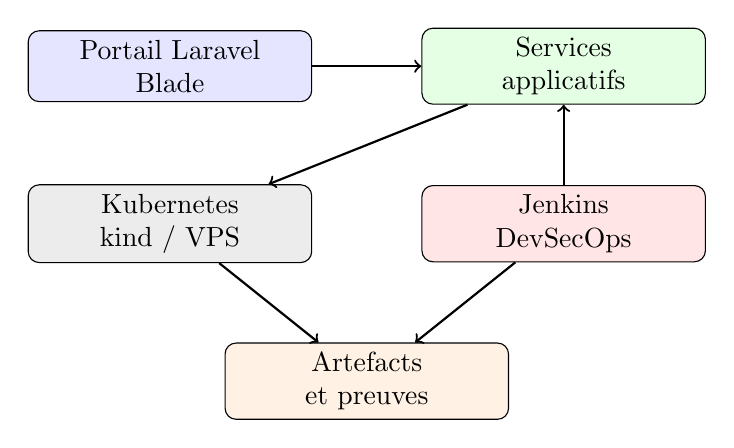
\begin{tikzpicture}[
        node distance=1.9cm,
        every node/.style={draw, rounded corners, align=center, minimum width=3.6cm, minimum height=0.9cm}
    ]
        \node[fill=blue!10] (portal) at (0,0) {Portail Laravel\\Blade};
        \node[fill=green!10] (services) at (5,0) {Services\\applicatifs};
        \node[fill=gray!15] (k8s) at (0,-2) {Kubernetes\\kind / VPS};
        \node[fill=red!10] (devsecops) at (5,-2) {Jenkins\\DevSecOps};
        \node[fill=orange!10] (proofs) at (2.5,-4) {Artefacts\\et preuves};

        \draw[->, thick] (portal) -- (services);
        \draw[->, thick] (services) -- (k8s);
        \draw[->, thick] (devsecops) -- (services);
        \draw[->, thick] (devsecops) -- (proofs);
        \draw[->, thick] (k8s) -- (proofs);
    \end{tikzpicture}
    \caption{Vue simplifiée de l’architecture SecureRAG Hub}
    \label{fig:vue_simplifiee_securerag}
\end{figure}

\subsection{Vue fonctionnelle}

La plateforme propose :

\begin{itemize}
    \item un portail utilisateur ;
    \item un portail administrateur ;
    \item une gestion des utilisateurs et des rôles ;
    \item un catalogue de chatbots métiers ;
    \item une préparation des conversations et de l’historique ;
    \item une supervision sécurité ;
    \item une vue DevSecOps pour présenter l’état des pipelines et des preuves.
\end{itemize}

\subsection{Vue technique}

Sur le plan technique, la solution repose sur :

\begin{itemize}
    \item Laravel Blade pour le portail web ;
    \item des services applicatifs métiers ;
    \item Docker pour la conteneurisation ;
    \item Kubernetes avec \texttt{kind} pour le déploiement local ;
    \item Kustomize pour la gestion des manifests ;
    \item Jenkins pour la CI/CD officielle ;
    \item Trivy, Syft, Cosign et Kyverno pour la sécurité ;
    \item une chaîne de preuves DevSecOps.
\end{itemize}

\subsection{Architecture microservices et principes de structuration}

L’architecture retenue pour \textit{SecureRAG Hub} repose sur une approche microservices. Ce choix ne répond pas uniquement à une préférence technologique, mais à une exigence de modularité, de maintenabilité et de séparation claire des responsabilités. Dans une plateforme de chatbots métiers sécurisés, plusieurs fonctions doivent coexister sans être confondues : l’authentification, la gestion des utilisateurs, la gouvernance RBAC, le catalogue de chatbots, l’historique conversationnel, l’audit et la supervision de la sécurité.

Une architecture monolithique aurait pu simplifier la première implémentation, mais elle aurait rapidement rendu plus difficile l’évolution différenciée des composants, la lisibilité de la solution et l’isolement des responsabilités. À l’inverse, l’approche microservices permet de découper la plateforme en services autonomes, chacun responsable d’un périmètre fonctionnel bien identifié.

Ce découpage présente plusieurs avantages pour le projet :

\begin{itemize}
    \item meilleure séparation des responsabilités fonctionnelles et techniques ;
    \item évolution plus simple d’un service sans impact direct sur l’ensemble de la plateforme ;
    \item lisibilité architecturale renforcée pour la soutenance ;
    \item adéquation avec une logique Kubernetes ;
    \item meilleure intégration à une démarche DevSecOps.
\end{itemize}

\subsection{Composants principaux de l’architecture}

\subsubsection{Portail web}

Le portail web constitue la couche de présentation du système. Il est développé avec Laravel Blade et permet de proposer une interface simple, maintenable et adaptée au contexte académique. Il offre des vues différenciées selon les profils, notamment pour les utilisateurs métiers et les administrateurs.

\subsubsection{Service d’authentification et de gestion des utilisateurs}

Ce service porte la logique d’authentification, de gestion des profils, des rôles et des permissions. Il constitue l’un des piliers de la gouvernance de la plateforme, car il contrôle l’accès aux fonctionnalités selon les profils définis.

\subsubsection{Service de gestion des chatbots}

Le service de gestion des chatbots administre le catalogue des assistants disponibles, leur configuration métier, leur domaine d’usage, ainsi que leur association à certaines règles de visibilité ou de sensibilité.

\subsubsection{Service de conversations}

Le service de conversations structure l’échange entre l’utilisateur et le chatbot. Dans la version actuelle, il prépare la gestion des conversations et l’historique, tout en laissant ouverte l’intégration future d’une orchestration IA plus avancée.

\subsubsection{Service d’audit et de supervision sécurité}

Ce service a pour rôle de conserver les traces, les événements significatifs, les incidents et les éléments de preuve nécessaires à la supervision. Il participe directement à la gouvernance et à la défendabilité technique du projet.

\subsubsection{Infrastructure d’exécution}

L’infrastructure locale repose sur Docker, un registre OCI local accessible depuis le cluster, un cluster Kubernetes \texttt{kind}, Kustomize pour la personnalisation des manifests, et Jenkins pour la chaîne CI/CD officielle. Cette infrastructure fait partie intégrante de la démonstration du projet, car elle montre la capacité à construire, valider, déployer et tracer la solution dans un environnement maîtrisé.

\subsection{Choix technologiques et justification}

Les choix technologiques retenus pour \textit{SecureRAG Hub} ont été guidés par quatre critères principaux : la stabilité de la démonstration, la lisibilité de l’architecture, la cohérence avec les objectifs du projet et la capacité à produire des preuves techniques exploitables.

\subsubsection{Laravel Blade}

Laravel Blade a été retenu pour le portail web afin de disposer d’une interface simple, maintenable et adaptée à un projet académique. Ce choix permet de limiter la complexité frontend tout en conservant une séparation claire entre présentation, logique applicative et services métiers.

\subsubsection{Laravel pour les services métiers}

Laravel a aussi été retenu pour les services métiers, notamment ceux liés à la gestion des utilisateurs, des rôles, du catalogue de chatbots, des conversations et de l’audit. Ce choix permet de bénéficier d’un framework structuré, d’un système de migrations, de modèles Eloquent, de contrôles de validation, de tests et de mécanismes d’autorisation intégrables dans une logique RBAC.

\subsubsection{Docker}

Docker est l'outil de conteneurisation retenu pour le projet. Il permet de construire des images reproductibles pour les différents composants et de réduire les écarts entre les environnements d’exécution.

\subsubsection{Kubernetes avec \texttt{kind}}

Kubernetes a été retenu pour refléter un mode de déploiement moderne fondé sur l’orchestration de conteneurs. L’usage de \texttt{kind} permet de reproduire localement un cluster Kubernetes sans dépendre d’une infrastructure cloud.

\subsubsection{Kustomize}

Kustomize est utilisé pour structurer les manifests Kubernetes en séparant une base commune et des overlays adaptés à différents scénarios. Cette approche améliore la maintenabilité des fichiers d’infrastructure et permet de distinguer clairement les environnements.

\subsubsection{Jenkins}

Jenkins a été retenu comme outil officiel de CI/CD. Ce choix vise à centraliser les tests, les scans de sécurité, les validations, les campagnes de démonstration et la production d’artefacts. Dans le projet, Jenkins ne constitue pas seulement un outil d’automatisation ; il fait partie intégrante de la preuve DevSecOps présentée en soutenance.

\subsubsection{Outillage de sécurité et supply chain}

Des outils comme Semgrep, Gitleaks, Trivy, Syft, Cosign et Kyverno permettent d’intégrer la sécurité à plusieurs niveaux du cycle de vie logiciel. Leur intérêt ne réside pas uniquement dans leur utilisation individuelle, mais dans leur complémentarité :

\begin{itemize}
    \item Semgrep permet l’analyse statique du code ;
    \item Gitleaks détecte les secrets exposés ;
    \item Trivy analyse les vulnérabilités et les configurations ;
    \item Syft génère les SBOM ;
    \item Cosign prépare la signature et la vérification des images ;
    \item Kyverno prépare des politiques d’admission Kubernetes.
\end{itemize}

L’ensemble de ces choix technologiques permet de construire une architecture cohérente, démontrable et extensible, tout en restant compatible avec les contraintes réelles du projet.

\subsection{Justification du scénario production-like}

Le scénario production-like est retenu comme scénario officiel car il permet de garantir une démonstration stable, reproductible et alignée avec l’état réel du projet. Il évite de faire dépendre la soutenance d’un téléchargement lourd de modèle IA, d’un moteur RAG complet ou d’une infrastructure externe.

Cette décision ne réduit pas la valeur technique du projet. Au contraire, elle permet de séparer clairement :

\begin{itemize}
    \item ce qui est opérationnel et validé ;
    \item ce qui est préparé pour évoluer ;
    \item ce qui dépend encore de l’environnement ;
    \item ce qui constitue une perspective future.
\end{itemize}

\subsection{Positionnement par rapport aux agents IA}

Les agents IA constituent une perspective intéressante pour automatiser certaines tâches complexes : analyse d’incidents, enrichissement de réponses, classification de conversations ou recommandation d’actions. Toutefois, ils ne sont pas intégrés comme dépendance centrale dans la première version du projet.

\begin{table}[htbp]
    \centering
    \begin{tabular}{|p{3cm}|p{3cm}|p{3cm}|p{5cm}|}
        \hline
        \textbf{Framework} & \textbf{Complexité} & \textbf{Approche} & \textbf{Intérêt potentiel} \\
        \hline
        LangGraph & Moyenne à élevée & Graphes d’états & Orchestration contrôlée de workflows IA \\
        \hline
        CrewAI & Basse à moyenne & Rôles spécialisés & Simulation d’équipes d’agents métiers \\
        \hline
        AutoGen & Moyenne & Conversation multi-agents & Collaboration entre agents pour résoudre un problème \\
        \hline
    \end{tabular}
    \caption{Comparaison de frameworks d’agents IA potentiellement intégrables}
    \label{tab:frameworks_agents}
\end{table}

Ces frameworks sont donc considérés comme des pistes d’évolution et non comme des composants obligatoires de la version démontrable.

%====================================================
\section{Langage et méthodologie de conception}

\subsection{Choix de la méthodologie de conception}

Dans le domaine informatique, une approche méthodique et une gestion efficace du projet sont essentielles pour atteindre les objectifs fixés. Les équipes de développement sont confrontées à des défis tels que la maîtrise du temps, la gestion des coûts, la qualité logicielle et la réduction des risques d’erreurs. Dans ce contexte, le choix d’une méthodologie adaptée constitue un facteur déterminant pour la réussite du projet.

Pour \textit{SecureRAG Hub}, la méthodologie retenue doit être compatible avec plusieurs caractéristiques du projet : un périmètre évolutif, une architecture technique diversifiée, une forte dimension de démontrabilité et des dépendances variables à l’environnement local. Ces contraintes rendent peu pertinente une approche strictement séquentielle.

\subsection{Pourquoi une approche agile}

Une approche agile permet de découper le projet en itérations courtes, chacune produisant un incrément vérifiable. Cette logique est particulièrement adaptée à \textit{SecureRAG Hub}, car elle permet de consolider progressivement la plateforme, de prioriser les fonctionnalités critiques et d’ajuster les choix techniques en fonction des contraintes rencontrées.

L’agilité facilite également l’intégration continue des retours, l’identification précoce des blocages et la production progressive de preuves techniques. Dans un projet de fin d’études, cette capacité à démontrer régulièrement l’avancement réel est particulièrement précieuse.

\subsection{Choix de Scrum}

Parmi les approches agiles, Scrum a été retenue comme cadre méthodologique principal. Ce choix se justifie par sa simplicité relative, sa forte structuration des rôles et des événements, ainsi que par sa capacité à organiser le travail en cycles courts appelés sprints.

Dans le cas de \textit{SecureRAG Hub}, Scrum permet de maintenir une vision claire du projet tout en conservant la souplesse nécessaire pour intégrer des ajustements techniques. Il favorise également la traçabilité de l’avancement, la production d’incréments vérifiables et la cohérence entre objectifs fonctionnels et contraintes techniques.

\subsection{Justification approfondie du choix de Scrum}

Le choix de Scrum ne repose pas uniquement sur sa popularité dans les projets logiciels, mais sur son adéquation avec la nature spécifique de \textit{SecureRAG Hub}. Le projet combine en effet plusieurs dimensions hétérogènes : développement web, APIs, microservices, infrastructure Kubernetes, sécurité applicative, CI/CD, documentation et préparation de la soutenance.

Scrum permet de structurer le travail en incréments courts et vérifiables. Cette organisation présente plusieurs avantages :

\begin{itemize}
    \item progression visible et mesurable ;
    \item stabilisation prioritaire des éléments critiques pour la démonstration ;
    \item adaptation aux contraintes environnementales ;
    \item documentation progressive ;
    \item cohérence entre ce qui est développé, validé et démontrable.
\end{itemize}

Dans ce projet, Scrum n'a pas été appliqué comme une méthodologie formelle indépendante du contexte, mais comme un cadre d’organisation permettant de réduire progressivement l’incertitude. Chaque itération a été orientée vers un résultat vérifiable : un composant fonctionnel, un manifeste applicable, une preuve de sécurité, un rapport d’exécution ou un artefact de soutenance.

\section{Les fondements de la méthodologie Scrum}

Scrum repose sur trois piliers fondamentaux : la transparence, l’inspection et l’adaptation.

\begin{itemize}
    \item \textbf{Transparence :} l’état réel du projet doit être visible et compréhensible par les parties concernées. Pour 	extit{SecureRAG Hub}, cela se traduit par l’usage de tableaux de tâches, de rapports de validation, de runbooks et de supports de preuve.
    \item \textbf{Inspection :} chaque incrément produit doit être régulièrement vérifié. Cette inspection se fait à travers des tests, des scans de sécurité, des vérifications Kubernetes et l’analyse des artefacts produits.
    \item \textbf{Adaptation :} lorsque des contraintes ou des problèmes apparaissent, l’équipe doit pouvoir ajuster rapidement ses priorités et ses choix. C’est notamment ce qui a motivé la stabilisation du scénario démontrable.
\end{itemize}

Scrum repose également sur des rôles bien définis : le \textit{Product Owner}, responsable de la vision du produit et de la priorisation du backlog ; le \textit{Scrum Master}, garant de la méthode ; et l’équipe de développement, chargée de produire les incréments techniques.

Dans un contexte académique ou individuel, ces rôles sont adaptés. Le porteur du projet assume généralement plusieurs responsabilités à la fois, tout en conservant la logique d’organisation, de priorisation et de validation propre à Scrum.

\section{Événements Scrum : catalyseurs de collaboration et d’amélioration}

Les événements Scrum structurent le déroulement du projet et favorisent une progression régulière.

\begin{itemize}
    \item \textbf{Sprint Planning :} permet de définir les objectifs de l’itération, de sélectionner les tâches prioritaires et de clarifier les livrables attendus.
    \item \textbf{Daily Scrum :} assure un suivi régulier de l’avancement, l’identification des blocages et l’ajustement rapide des priorités.
    \item \textbf{Sprint Review :} permet de présenter l’incrément réalisé et de vérifier sa conformité avec les objectifs.
    \item \textbf{Sprint Retrospective :} sert à analyser les difficultés rencontrées et à améliorer la méthode de travail pour les itérations suivantes.
\end{itemize}

Dans \textit{SecureRAG Hub}, ces événements ne sont pas seulement des formalités méthodologiques. Ils servent à maintenir la cohérence entre l’architecture, les exigences de sécurité, la progression du portail, la stabilité du déploiement local et la préparation de la soutenance.

\section{Application de Scrum au projet SecureRAG Hub}

La méthodologie Scrum a été appliquée au projet sous forme d’itérations successives. Chaque sprint devait produire un livrable vérifiable : un service testable, un écran fonctionnel, un script exécutable, un manifeste Kubernetes applicable, un rapport de sécurité ou un document de preuve.

Cette contrainte a permis d’éviter une progression purement théorique et d’assurer une validation régulière de l’avancement. L’application de Scrum au projet a également facilité la hiérarchisation des priorités : d’abord la stabilité du scénario de démonstration, ensuite la structuration de la chaîne DevSecOps, puis l’enrichissement progressif des composants applicatifs.

Le backlog du projet a été organisé selon plusieurs niveaux de priorité :

\begin{itemize}
    \item les éléments indispensables à une soutenance stable ;
    \item les éléments renforçant la crédibilité fonctionnelle et technique de la plateforme ;
    \item les améliorations structurantes dépendant davantage du temps et de l’environnement.
\end{itemize}

Cette organisation a permis d’adapter en permanence la trajectoire du projet sans perdre de vue l’objectif principal : proposer une plateforme démontrable, cohérente et défendable.

\subsection{Microservices, communication inter-services et gouvernance technique}

Dans une architecture microservices, la qualité de la solution dépend du découpage fonctionnel mais aussi de la manière dont les services communiquent, sont déployés et sont gouvernés. Dans \textit{SecureRAG Hub}, cette dimension est particulièrement importante, car la plateforme combine des composants web, des services métiers et une infrastructure DevSecOps.

La communication entre services repose principalement sur des APIs REST, ce qui permet de maintenir des contrats lisibles et de faciliter l’intégration progressive des composants. Ce choix est cohérent avec la portée académique du projet, car il rend les interactions plus explicites et plus simples à documenter.

Sur le plan du déploiement, chaque service est conteneurisé afin d’être intégré à une logique uniforme d’exécution sur Kubernetes. Cette homogénéité facilite l’automatisation dans Jenkins, les scans de sécurité, la production de SBOM et la démonstration des preuves runtime.

Sur le plan de la gouvernance, l’architecture microservices impose également une réflexion sur :

\begin{itemize}
    \item la séparation des responsabilités ;
    \item la cohérence des contrats d’API ;
    \item la gestion des secrets et des configurations ;
    \item l’isolation réseau entre composants ;
    \item la traçabilité des déploiements et des validations.
\end{itemize}

Même si toutes ces dimensions ne sont pas encore exploitées au même niveau de maturité dans la version actuelle, elles structurent déjà les choix d’architecture et renforcent la crédibilité globale de la plateforme.

%====================================================
\section{Bénéfices attendus et perspectives}

\subsection{Bénéfices attendus}

Les bénéfices attendus de \textit{SecureRAG Hub} sont les suivants :

\begin{itemize}
    \item fournir une plateforme claire pour gérer des chatbots métiers ;
    \item sécuriser l’accès aux fonctionnalités par rôles ;
    \item démontrer une chaîne DevSecOps crédible ;
    \item produire des preuves exploitables pour l’évaluation ;
    \item disposer d’une base évolutive pour intégrer un véritable moteur RAG ;
    \item réduire les risques liés à une démonstration dépendante d’un LLM lourd ;
    \item renforcer la traçabilité des versions déployées et des artefacts produits.
\end{itemize}

Au-delà de ces bénéfices immédiats, le projet contribue également à structurer une démarche d’ingénierie réutilisable. En articulant portail web, sécurité, déploiement local et gouvernance, il offre un socle conceptuel et technique pouvant servir de base à des extensions futures plus ambitieuses.

\subsection{Perspectives}

Les principales perspectives d’évolution sont les suivantes :

\begin{itemize}
    \item connecter davantage les écrans Blade aux services persistants ;
    \item compléter les services de conversation et d’audit ;
    \item formaliser les contrats OpenAPI ;
    \item intégrer un moteur RAG réel ;
    \item renforcer l’observabilité ;
    \item poursuivre l’industrialisation GitOps ;
    \item renforcer les politiques Kyverno en mode \texttt{Enforce} ;
    \item intégrer progressivement une gestion avancée des secrets.
\end{itemize}

Ces perspectives montrent que le projet ne doit pas être interprété comme un démonstrateur figé, mais comme une base structurée capable d’évoluer vers une plateforme plus complète.

%====================================================
\section{Conclusion}

Cette étude préalable a permis de clarifier le contexte, la problématique, les objectifs, le périmètre et les limites du projet \textit{SecureRAG Hub}. Elle montre que le projet ne se limite pas à la création d’un chatbot, mais qu’il vise la conception d’une plateforme complète intégrant portail web, services applicatifs, gouvernance RBAC, Kubernetes local et chaîne DevSecOps.

L’analyse des besoins, des usages et des risques a mis en évidence que la valeur du projet réside autant dans la qualité de son encadrement architectural que dans la logique conversationnelle qu’il prépare. L’analyse de l’existant a également permis de situer le projet par rapport aux solutions du marché et de mettre en évidence sa valeur spécifique : la combinaison entre architecture modulaire, sécurité, industrialisation et démonstration locale reproductible.

Le choix d’une méthodologie Scrum illustre la volonté de structurer le projet selon une approche claire, progressive et défendable. Les prochains chapitres détailleront la conception, la mise en oeuvre, l’intégration des mécanismes de sécurité et l’évaluation de la solution retenue.

